%Geometrické a objemové modelování. Hraniční metoda, metoda CSG, výčet prostoru, oktantové stromy.

\subsection{Geometrické a objemové modelování}
\begin{itemize}
	\item Geometrické modelování zkoumá reálné objekty z hlediska geometrických vlastností.
	\item Je to soubor metod k popisu těles. \\ Typy modelů
	\item Objemové modely (volume, solid model) -- Jedná se o modely, které v sobě zahrnují informace o části prostoru, kterou těleso zaujímá. Pro popis objemového modelu se používají tyto způsoby:
	\begin{itemize}
		\item \textbf{B--reprezentace s orientovanými stěnami} -- objemový model může být určen seznamem orientovaných stěn (B--reprezentace), které dané těleso ohraničují (stěny mohou být rovinné i nerovinné -- viz hraniční modely). Stěna je orientována, jestliže můžeme jednoznačně určit, která strana stěny je vnitřní a která je vnější vzhledem k danému tělesu.
		\item \textbf{CSG reprezentace} -- modelované těleso je reptezentováno binárním stromem, jehož vnitřní uzly představují množinové operace nebo geometrické transformace a listy představují elementární tělesa (primitiva). V poslední době se staly oblíbenými hybridními modely, které v sobě uchovávají současně CSG i B--reprezentace.
		\item \textbf{Dekompoziční reprezentace} -- model je určen seznamem objemových elementů (např. krychliček), které dané těleso vyplňují -- např octree reprezentace
\end{itemize}
\end{itemize}

\subsubsection{Drátěné (hranové) modely (wireframe model)}
\begin{itemize}
	\item Drátěné modely jsou reprezentovány hranami objektu a skládají se z bodů, přímek a křivek.
	\item První wireframe systémy byly pouze dvou-dimenzionální.
	\item Používaly se především na návrhy tištěných spojů.
	\item Základními elementy těchto systémů byly body, přímky a oblouky některých kuželoseček.
	\item Vnitřní reprezentaci tvořil obvykle seznam úseček a oblouků.
	\item V 70. letech byla wireframe reprezentace použita i pro modelování v prostoru. Zde však vznikaly dost závažné problémy:
	\begin{itemize}
		\item možnost vytvoření nejednoznačných modelů
		\item možnost vytvoření nesmyslných modelů
		\item problém velkého počtu dat pro "drátěný" popis objektu
	\end{itemize}
	\item Průmět drátěného modelu může mít více významů.
	\item Pokud u modelu vynecháme některé hrany, dostaneme nesmyslný (nonsense) model.
	\item U wireframe modelů je velice obtížné kontrolovat jejich logickou správnost.
	\item Poslední nevýhodou je značné množství dat, které jsou nutné pro úplný popis objektu. 
	\item Například obecně pro jednoznačné určení kvádru v prostoru stačí výška, šířka, hloubka a poloha.
	\item Wireframe model kvádru musí obsahovat souřadnice osmi vrcholů, musí být určeno dvanáct hran a ještě není model jednoznačný.
\end{itemize}

 \subsection{Hraniční (povrchové) modely B--reprezentace}
 \begin{itemize}
 	\item Tato reprezentace patří k nejpoužívanějším typům při geometrickém popisu objektů.
 	\item Metoda reprezentace tělesa pomocí hranice, spočívá v tom, že těleso je dáno svou hranici (povrchem), která je orientována a dělí tedy prostor na dvě části - vnitřek tělesa a vnějšek tělesa.
 	\item Popis tělesa rozdělen na dvě části:
 	\begin{itemize}
		\item \textbf{topologická} - popisuje vzájemné vztahy mezi entitami tělesa (vztahy mezi stěnami, hranami a vrcholy)
		\item \textbf{geometrická} - popisuje umístění entit tělesa v prostoru (souřadnice prostorů, rovnice ploch, ...)
 	\end{itemize}
 	\item Těleso je definováno těmito informacemi:
 	\begin{itemize}
		\item	\textbf{seznam povrchů (shell)}, které těleso omezují
		\item	\textbf{seznam stěn (face)} definující povrch tělesa
		\item	\textbf{seznam smyček (loop)}, které definují stěny. Jde o orientované hrany. Obsahuje-li stěna jednu smyčku, jde o stěnu bez děr. Je li dána více smyčkami jsou ve stěně tunely. Směr rotace smyčky udává 	normálu stěny a určuje tedy na které straně stěny je vnitřek tělesa a která strana je vnější (smyčka proti směru hodinových ručiček – stěna z vnějšku). Je‑li uprostřed stěny, jde o díru (tunel)
		\item	\textbf{seznam hran (edge)} definující smyčky
 	\end{itemize}
 	\item Těleso nesmí být definováno všemi dohromady, aby nedocházelo k nekonzistenci informací.
 	\item Proto se uchovávají jen některé z těchto informací a další se dopočtou.
 	\item Jednou z hraniční reprezentací těles je datová struktura zvaná okřídlená hrana daná hranou a dvěma plochami k ní přiléhajícími.
 \end{itemize}

 \subsection{Metoda CSG}
 \begin{itemize}
 	\item \textbf{Constructive Solid Geometry} je metoda reprezentace těles, kdy jsou tělesa tvořena za pomocí standardních primitivních těles (kvádr, hranol, válec, kužel, koule, toroid, …), regularizovaných booleovských operací a geometrických transformací.
	\item Uživatel si naskládá primitivní (či dříve vytvořené) tělesa do prostoru a aplikuje na ně boolovské operace jako sjednocení, průnik, rozdíl, čímž vznikne nový útvar.
	\item Z hlediska \textbf{datové struktury} jsou tělesa popsány stromem. Listy stromu odpovídají primitivním tělesům a transformacím, vyčteme z nich tedy rozmístění a velikosti těles. Zbylé uzly tvoří boolovské operace které jsou nad tělesy vykonány.
	\item CSG strom je binární, pokud chápeme boolovské operace jako binární, jinak tomu být nemusí.
		\begin{figure}[H]
		\centering
		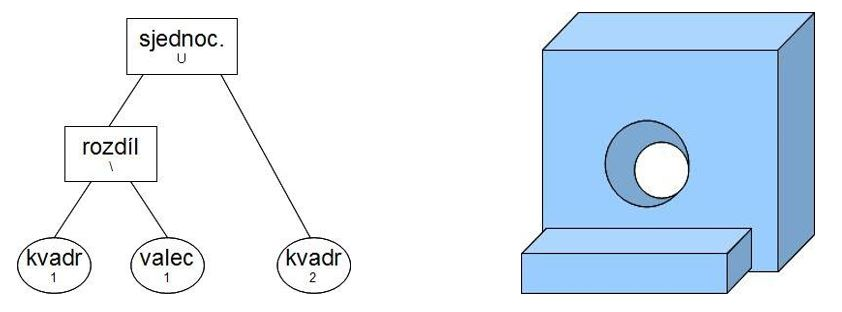
\includegraphics[width=0.6\textwidth]{assets/4_csg}
		\end{figure}
 	\item Výhoda stromové struktury je že uchovává historii modelace tělesa, kterou lze využít při další úpravě.
 	\item Další výhodou CSG tohoto přístupu je jednoduchost boolovských operací.
 	\item Na rozdíl od hraniční metody, není třeba náročného výpočtu hranic nového tělesa.
 \end{itemize}

 \subsection{Výčet prostoru}
 \subsection{Oktanové stromy}
 \begin{itemize}
 	\item Je jedna z metod objemového modelování.
 	\item Těleso je definováno \textbf{objemovými elementy} (\textbf{voxel}), což je něco jako 3D pixel.
 	\item Jde o malé krychličky, na které je rozdělen prostor a které buď jsou v tělese nebo nejsou.
 	\item Na obrázku níže je zobrazen tento způsob pro 2D. Zápis takového 2D tělesa by mohl vypadat takto: [0, 0, false], [0, 1, true], [0, 2, true], ...
	\item Čím jemnější detaily potřebujeme modelovat, tím jemněji potřebujeme plochu rozdělit.
	\item Jenže tím se nám taky zvedají nároky na paměť. Proto zavádíme oktanové stromy, které tento problém eliminují.
		\begin{figure}[H]
		\centering
		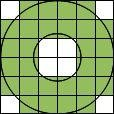
\includegraphics[width=0.4\textwidth]{assets/4_octan}
		\end{figure}
	\item Oktantové stromy zmenšují paměťovou náročnost detailních modelů, tak že zjemní pouze elementy, kterých se detail týká.
	\item Začíná se tedy na velkých voxelech, ale ty nyní mohou nabývat třech stavů:	
	 \begin{itemize}
			\item voxel je obsažen v tělese
			\item voxel není obsažen v tělese
			\item voxel je částečně obsažen v tělese.
	\end{itemize}
	\item V dalším kroku se řeší ty voxely, které jsou nerozhodné, tedy částečně obsaženy v tělese.
	\item Takový voxel ležící na hranici tělesa rozdělíme na osm menších voxelů.
	\item Na obrázku níže je tento postup znázorněn ve 2D prostoru.
		\begin{figure}[H]
		\centering
		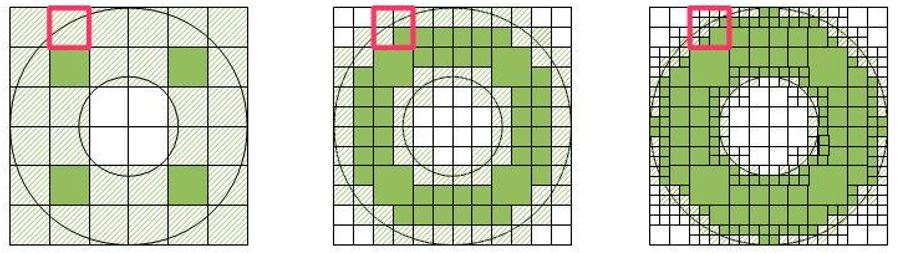
\includegraphics[width=0.6\textwidth]{assets/4_octan2}
		\end{figure}
	\item Výsledná struktura je pak zapsána do oktanových stromů (stromy s max. osmi větvemi).
	\item Vpravo máme oktanový (respektive kvartálový, protože jsme jen v 2D prostoru) strom popisující oblast, která je vyznačená červeně na obrázku výše.
		\begin{figure}[H]
		\centering
		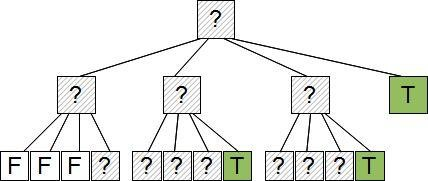
\includegraphics[width=0.6\textwidth]{assets/4_octan_struct}
		\end{figure}
\end{itemize}
